%!TEX root = ../06-Ideal-And-Real-Gases.tex
\chapter{Vapor Pressure Curve Of N-Hexane}
This exerpiment explores the evaporation enthalpy of n-hexane and its associated vapor pressure curve.

\section{Theory}
\begin{figure}[tbp]
	\centering
	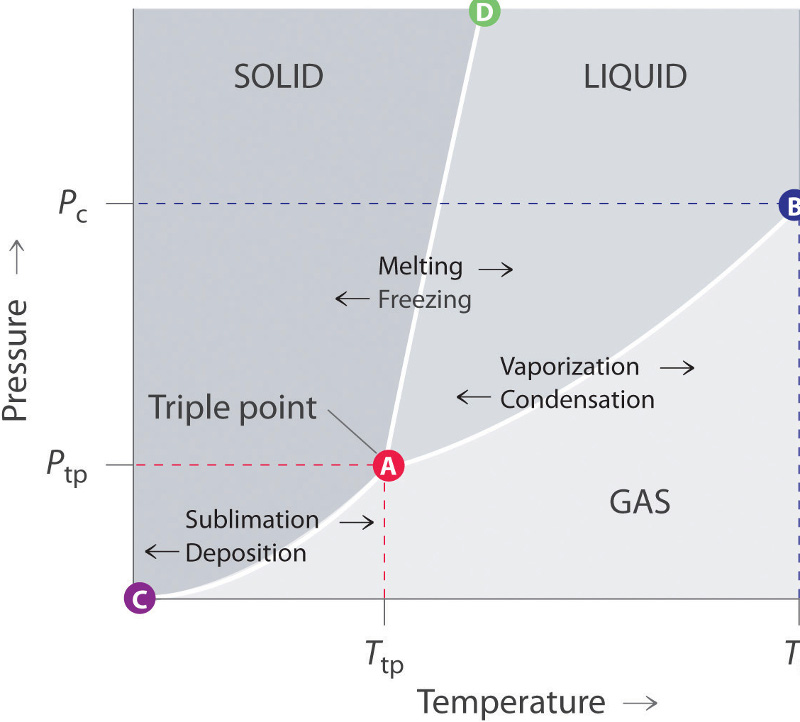
\includegraphics[width=.4\textwidth]{./img/phase.jpg}
	\caption[Phase diagram of n-hexane]{\textbf{Phase diagram of n-hexane} The vapor pressure curve can be seen between the gaseous and liquid phase\newline Source:\url{saylordotorg.github.io/text_general-chemistry-principles-patterns-and-applications-v1.0/s15-07-phase-diagrams.html}}
	\label{fig:n_hexane_phase_diagram}
\end{figure}

A container filled with n-hexane is placed inside of a water bath.
The water bath is heated up and let cool down afterwards.
During both processes, the vapor pressure $p$ and temperature $T$ are measured in regular intervals.

\autoref{fig:n_hexane_phase_diagram} shows the phase diagram of n-hexane.
Unlike water, it is a substance which does not show negative thermal expansion.
The curve between liquid and vapor phase is called the vapor pressure curve.
Points on it are in phase equilibrium, which means that the same amount of vapor condensates as water evaporates.

Using \texttt{Clausius-Clepeyron}'s equation, the evaporation enthalpy $\Lambda$ can be calculated as
\begin{align}\label{eq:evap_enth}
	\Lambda&=T\cdot\left(V_\text{g}-V_\text{l}\right)\cdot\frac{\d p}{\d T} \nonumber \\
	&=TV_\text{g}\cdot\frac{\d p}{\d T}\quad(V_\text{g}\gg V_\text{l})
\end{align}
where $V_\text{g}$ and $V_\text{l}$ denote the gaseous and liquid volume respectively.

Using the ideal gas law, $V_\text{g}$ can be expressed as
\begin{equation}\label{eq:gas_law}
	V_\text{g}\at[\bigg]{n=1}=\frac{RT}{p},
\end{equation}
where $R$ is the universal gas constant $(=\SI{8.31}{\joule\per\mole\kelvin}$).

Combining equations \ref{eq:evap_enth} and \ref{eq:gas_law}, we get the differential equation
\begin{equation}\label{eq:dgl}
	\Lambda=\frac{RT^2}{p}\cdot\frac{\d p}{\d T}.
\end{equation}
Solving \autoref{eq:dgl} yields
\begin{align}
	\frac{\Lambda}{T}&=-R\cdot\log{p}+\text{const.} \nonumber \\
	\Leftrightarrow\ \log{p}&=-\frac{\Lambda}{R}\cdot \frac{1}{T} + \text{const.}	\label{eq:fit_eq} \\
	\Leftrightarrow\ y&=a\cdot x + \text{const.} \nonumber
\end{align}

$\Lambda$ can be determined by fitting this linear model to acquired data $(\frac{1}{T},p)$.

\section{Evaluation}
\begin{figure}[tbp]
	\centering
	\begin{subfigure}{0.4\textwidth}
		\centering
		\includegraphics[width=.9\linewidth]{./data/plots/4_vapor.pdf}
		\caption{\textbf{Measured vapor pressure curve of n-hexane}}
		\label{subfig:press_curve_meas}
	\end{subfigure}
	\begin{subfigure}{0.4\textwidth}
		\centering
		\includegraphics[width=.9\linewidth]{./data/plots/4_enth.pdf}
		\caption{\textbf{Linear regression for determining $\Lambda$}}
		\label{subfig:lambda_meas}
	\end{subfigure}
	\caption{Measured Vapor Pressure of n-Hexane}
\end{figure}

No errors can be estimated as both measurements $T$ and $p$ have negligable uncertainties.
$T$ is measured with a highly precise, electronic thermometer and the differential height of the manometer's filament $\Delta h$, which is proportional to $p$, is measured with a telescope.
\autoref{subfig:press_curve_meas} shows the measured vapor pressure curves.
\autoref{subfig:lambda_meas} shows the linear regression for determining $\Lambda$.
Fitting the model in \autoref{eq:fit_eq} to the data yields the parameters
\begin{align*}
	a_\text{cool}=\SI{-1701(297)}{\kelvin},\ a_\text{heat}=\SI{-1605(274)}{\kelvin},
\end{align*}
with $R^2$-values of
\begin{align*}
	R^2_\text{cool}=\num{0.99},\ R^2_\text{heat}=\num{0.99},
\end{align*}
so the model describes the data in an overly sufficient manner.
These slopes yield enthalpy of vaporization coefficients of
\begin{align*}
	\Lambda_\text{cool}&=\SI{14.14(25)}{\kilo\joule\per\mole},\ \Lambda_\text{heat}=\SI{13.34(23)}{\kilo\joule\per\mole}, \\
	\Rightarrow\ \overline{\Lambda}&=\SI{13.74(12)}{\kilo\joule\per\mole}.
\end{align*}
This value deviates from the literature value\footnote{\url{de.wikipedia.org/wiki/N-Hexan}} of $\Lambda_\text{lit}=\SI{28.85}{\kilo\joule\per\mole}$ by \num{52}\%.
This deviation can be explained by the literature value being specified at the normal pressure boiling point, which was not attained in this experiment.
